\documentclass{article}
\usepackage[T1]{fontenc}  
\usepackage[scaled=0.82]{beramono}  
\usepackage{microtype} 
\usepackage{amsmath}
\usepackage{amsfonts}
\usepackage{mathtools}
\usepackage{bm}
\usepackage{slashed}
\usepackage{amssymb}
\usepackage{hyperref}
\usepackage{nameref}
\usepackage{siunitx}
% \usepackage[backend=bibtex]{biblatex}
\usepackage[margin=2cm]{geometry}
% \addbibresource{matching-pursuit.bib}

\DeclareMathOperator{\E}{E}

\title{Study on MCP-PMT Mechanism based on secondary electron emission}
\author{Jun,Weng; Zhang, Aiqiang; Xu, Benda; \\ Center for High Energy Physics}
\date{\today}

\begin{document}
\maketitle
\section{The long-tail in MCP-PMT charge response }\label{sec:long-tail}
\subsection{Single photoelectron charge response}\label{subsec:statistical}
The charge response of PMT when it works at photon counting mode can be discribed as Gaussian distributions discribed as \refeq{eq:sreal}~\cite{1994Absolute}
\begin{equation}
    \begin{aligned}
        Q_{\text {real }}(x) \approx & \left \{\frac{(1-w)}{\sigma_0 \sqrt{2 \pi}} \exp \left(-\frac{\left(x-Q_0\right)^2}{2 \sigma_0^2}\right)+w \theta\left(x-Q_0\right) \times \alpha \exp \left[-\alpha\left(x-Q_0\right)\right]\right\} \mathrm{e}^{-\mu}\\
        &+\sum_{n=1}^{\infty} \frac{\mu^n \mathrm{e}^{-\mu}}{n !}  \times \frac{1}{\sigma_1 \sqrt{2 \pi n}}  \times \exp \left(-\frac{\left(x-Q_0-Q_{\text {sh }}-n Q_1\right)^2}{2 n \sigma_1^2}\right)
    \end{aligned}
    \label{eq:sreal}
\end{equation}
From \refeq{eq:sreal}, the charge response is discribed as the Gaussian distributions, whose mean value represents the number of photoelectrons produced by the photon at the photocathode a process known as the Poisson process.
When the trigger rate $\mu$ is less than 0.1, the probability of producing two or more photoelectrons is less than one tenth of the probability 
of producing one photoelectron, and the PMT charge response is left with two Gaussian peaks as~\ref{fig:spe_sreal}.
\begin{figure}[ht]
    \centering
    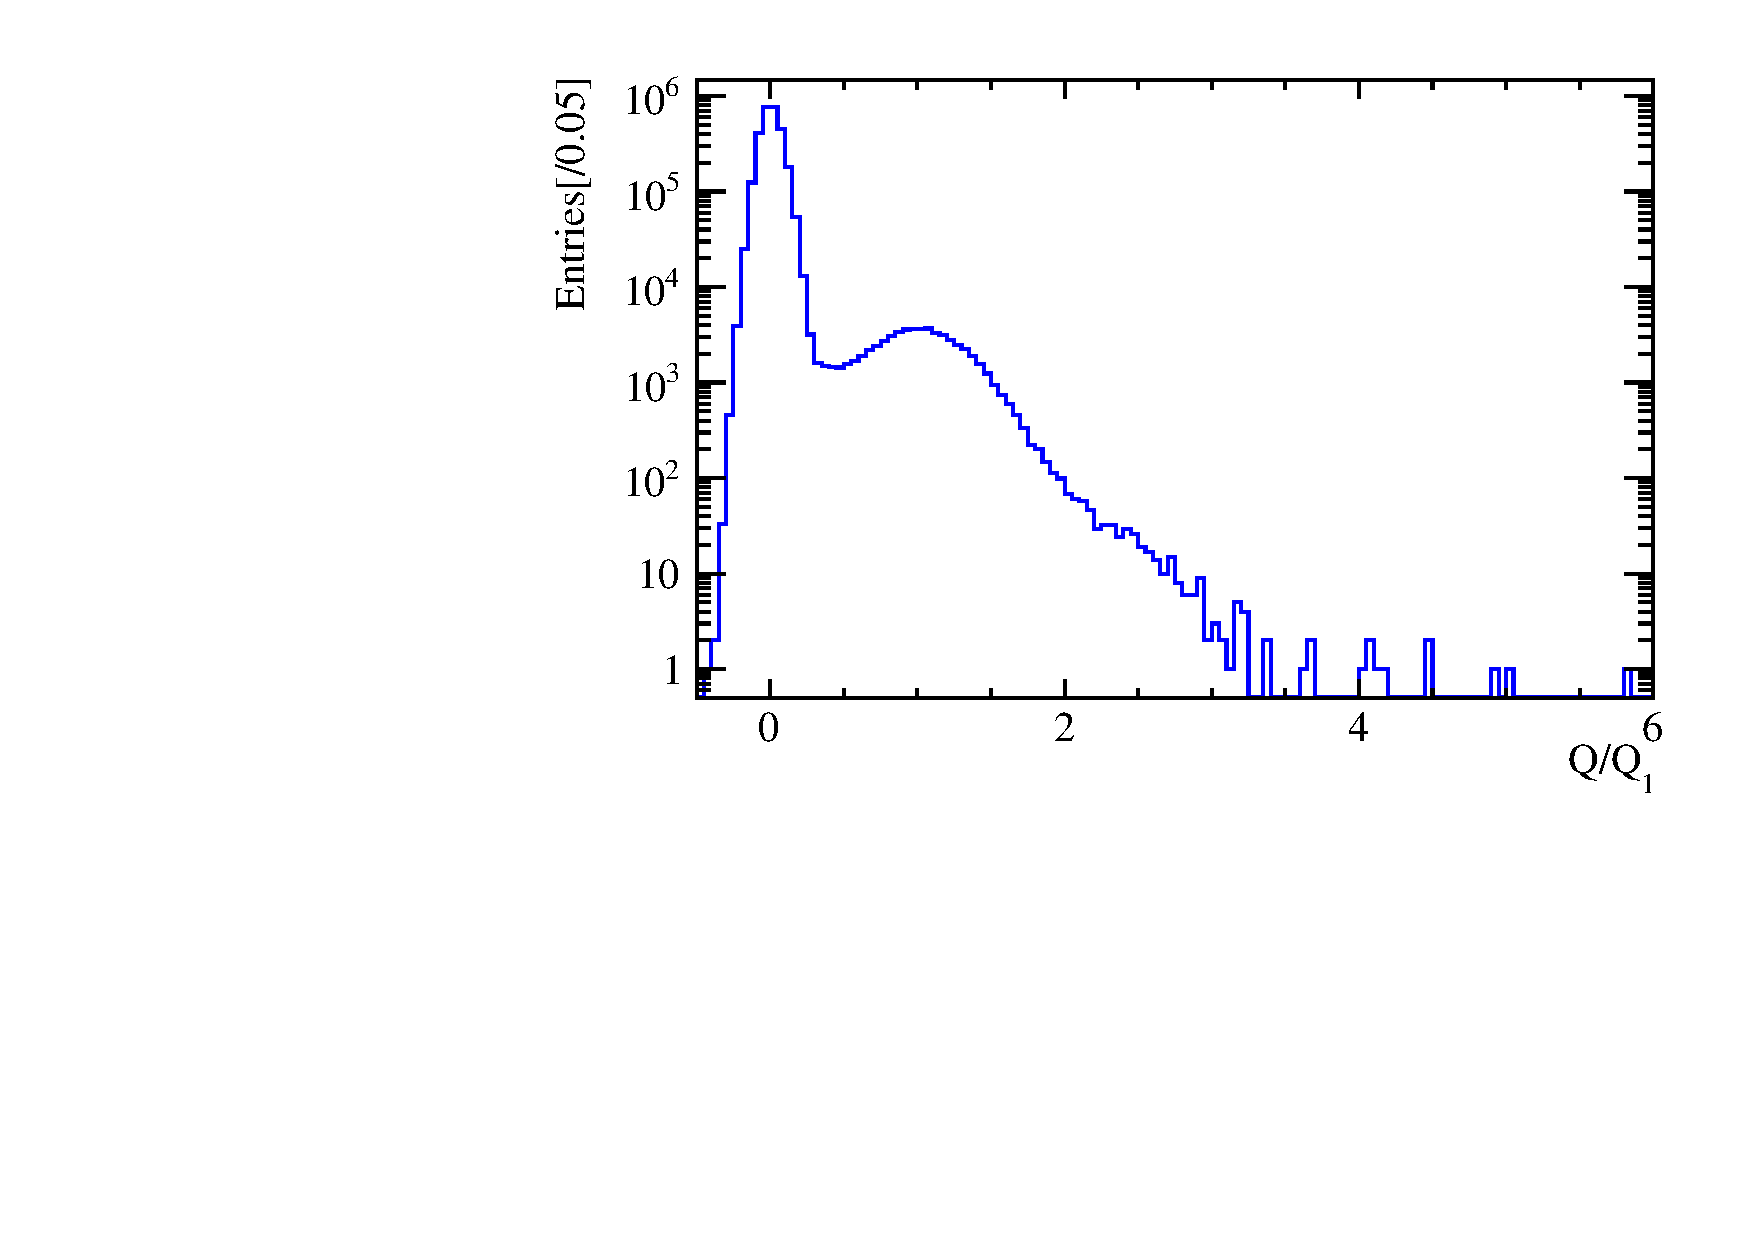
\includegraphics[height=7cm]{pic/siglepe.pdf}
    \caption{Single photoelectron charge response of Hamamatsu CR365}\label{fig:spe_sreal}
\end{figure}
\subsection{long tail in MCP-PMT charge response}\label{subsec:tail}
In the performance tests to evaluate MCP-PMT used by JNE, we found a long tail in the charge spectrum of MCP-PMTS in the single photoelectron mode as shown in Fig~\ref{fig:tail}
\begin{figure}[ht]
    \centering
    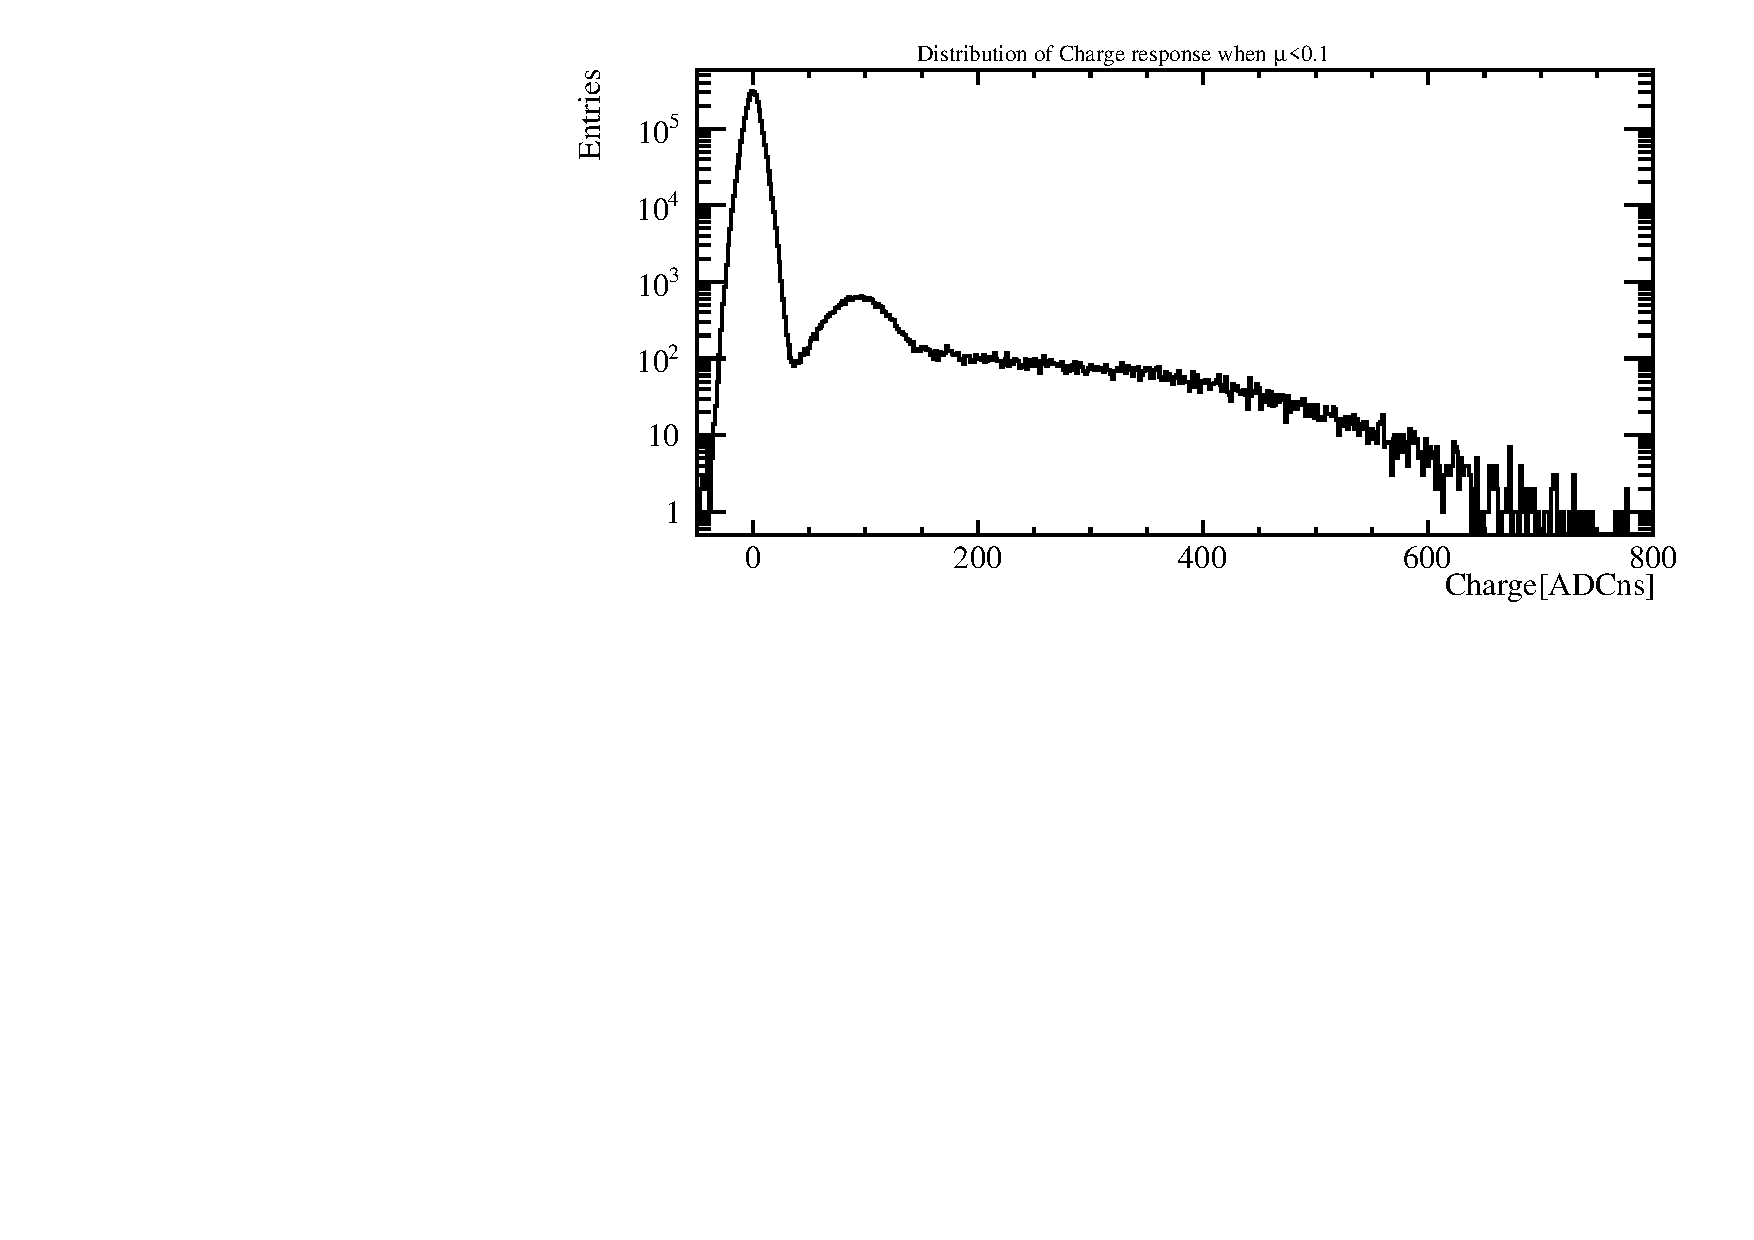
\includegraphics[height=7cm]{pic/longtail.pdf}
    \caption{Single photoelectron charge response of MCP-PMT PM2112-9089F}\label{fig:tail}
\end{figure}
\section{Statistical model of MCP-PMT charge response}
\subsection{The structure of MCP-PMT}\label{subsec:structure}
When the photon reaches the photocathode, it is converted into photoelectron through photoelectric conversion
Under the action of electric field, it reaches the microchannel plate~(MCP). The microchannel plate is coated with secondary emission material of certain thickness.
The electrons interact with the surface of the microchannel plate to generate multiple electrons. 
These electrons interact with the surface of the microchannel plate continuously under the action of electric field to form multiple electrons.
Finally, they reach the anode to form electrical signals that can be directly measured.
\begin{figure}[ht]
    \centering
    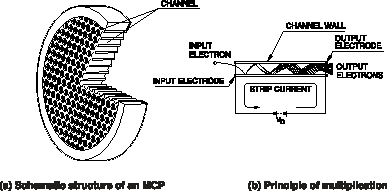
\includegraphics[height=5cm]{pic/structure.pdf}
    \caption{After entering the MCP hole, the electron collides with the shannel wall for many times and multiplies in a cascade process}\label{fig:structure}
\end{figure}

In fact, when electrons reach the upper surface of the MCP, 
they may enter the MCP channel directly and undergo a cascade multiplication process, 
which is described in Fig~\ref{fig:structure}. 
It may also collide with the upper face of the MCP.\@

In order to improve the collection efficiency, 
the MCP end face of the McP-pmt used by JNE is coated with a layer of secondary emission material.
Therefore, the electrons hit on the upper face of MCP can also enter the MCP hole for multiplication 
under the action of electric field after collision. This means that MCP-PMT can work in two modes, 
and each photoelectron can only be amplified in one of these modes. We define the mode that directly enter  the channel for multiplication as \textit{channel mode} and   
the mode that enters the channel for multiplication after colliding with the upper surface as \textit{surface mode}.
\begin{figure}[ht]
    \centering
    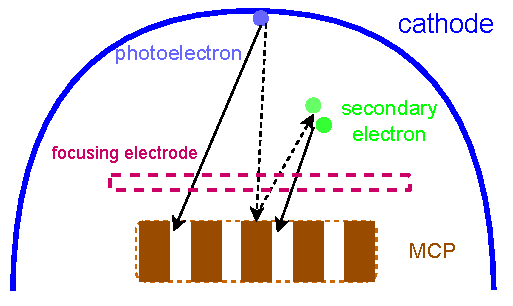
\includegraphics[height=5cm]{pic/MCPelectron.pdf}
    \caption{The photoelectrons directly enter the channel and enter the channels after hitting the upper face of the MCP}\label{fig:MCP}
\end{figure}
\subsection{double gamma model}\label{subsec:doublegamma}
Considering two multiplication modes, both of which multiply a single electron by a factor of $10^7$, 
Their corresponding charge response can be described by Gaussian distribution respectively. 
These two modes are mixed together in proportion to form the single photoelectronic response of MCP-PMTs as \refeq{eq:doublegaus}
\begin{equation}
    \label{eq:doublegaus}
    \begin{aligned}
        & Q_{MCP-PMT} = p\times Q_{channel\  mode} + (1-p)\times Q_{surface\  mode} \\
        & Q_{channel\  mode} \sim \mathcal{N} (\mu_1, \sigma_1) \\
        & Q_{surface\  mode} \sim \mathcal{N} (\mu_2, \sigma_2)
    \end{aligned}
\end{equation}
Use double Gaussian distribution to fit the charge response:

\subsection{dark noise from MCP}\label{subsec:dnr}

\subsection{secondary electron emission}\label{subsec:fuman}
Photoelectrons are produced with very little energy, about the size of a few electronvolts, and the energy arriving at MCP is determined primarily by the electric field.
When the photoelectron is multiplied in channel mode, the energy entering the channel is the energy accelerated by the electric field, which is about \SI{600}{eV}. 
Different from channel mode, the energies of electrons entering the channel is complicated, 
and we use Fuman Model to discribe the energy distribution of secondary electrons\cite{2002Probabilistic}. 

\subsection{Gain at low incident energy}\label{sec:gain}



\section{secondary electron emission affects TT distribution}\label{sec:TT}
\newpage
\bibliographystyle{plain}
\bibliography{ref}

\end{document}